\documentclass[letterpaper, 12pt]{report} % for letter size paper
% 215.9mm × 279.4mm

\usepackage{ifxetex}
\usepackage[T1]{fontenc}
\usepackage[utf8]{inputenc}

\usepackage[french]{babel}
\usepackage{tikz, background, titling, kantlipsum, setspace}
\usepackage[left=1.5in,right=0.5in,top=0.98in,bottom=.525in]{geometry}

\usepackage{mathrsfs}
\usepackage{textpos}

\usetikzlibrary{calc}
\usetikzlibrary{shapes}
\usetikzlibrary{backgrounds}
%\tikzstyle{block} = [rectangle, draw, fill=blue!20, text width=5em, text centered, rounded corners, minimum height=4em] 
\tikzstyle{line} = [draw, text centered]
%\tikzstyle{output} = [fill=white]

\definecolor{textcolorPencil}{rgb}{0.99,0.69,0.07}


\newcommand{\stardelimiter}{{\begin{center}\vspace{0.3cm} $\star \star \star$\vspace{0.25cm}\end{center}}}

\newcommand{\datemarge}[1]{%
    \begin{textblock}{3}(-3.1,0)
        {\color{blue}#1}
    \end{textblock}
}

%\renewcommand{\rmdefault}{augie}
%\fontfamily{French Cursive}
\usepackage{frcursive}
\DeclareTextFontCommand{\helvetica}{\fontfamily{phv}\selectfont}
\renewcommand{\rmdefault}{frc}

\title{Quand la logique s'en mêle}
\author{Alexandre Janniaux}

\begin{document}
  %\pagestyle{empty}
\doublespacing{}
  %\kant[1-6]{}

  \maketitle

  \backgroundsetup{%
 angle=0,
 scale=1,
 placement=bottom,
 contents={%
     \begin{tikzpicture}[overlay]%
         [
             normal line/.style={gray, very thin},
             every node/.append style={black, align=center, opacity=1}
         ]
         \begin{scope}[on background layer]
             %\foreach \y in {1,2,...,10} {
             %  \draw[line] (0,0.71\y) -- (8.5in,0.71\y);
             %}
             %\node (t) [font=\LARGE, anchor=south] at ($(0,25.56)!1/2!(8.5in,25.56)$) {\thetitle};
             %\node (d) [font=\large, anchor=south west, xshift=1.5em] at (0,25.6) {\today};
             %\node (p) [font=\large, anchor=south east, xshift=-1.5em] at (8.5in,25.56) {p.~\thepage};
%             \draw[line,color=red] (1.16in,0) -- (1.16in,23in);
             \draw[line width=0.3pt,color=gray,step=0.5cm] (current page.south west) grid (current page.north east); % (0,-13in) grid (10in,10in);
             %\draw[line width=0.5pt] (0,1.4in) (10in,1.4in);
             %\foreach \y in {0.71,1.41,...,25.56}
             %  \draw[normal lines] (0,\y) -- (8.5in,\y);
             %\draw[normal lines] (1.25in,0) -- (1.25in,11in);
             %\node (t) [font=\LARGE, anchor=south] at ($(0,25.56)!1/2!(8.5in,25.56)$) {\thetitle};
             %\node (d) [font=\large, anchor=south west, xshift=1.5em] at (0,25.6) {\today};
             %\node (p) [font=\large, anchor=south east, xshift=-1.5em] at (8.5in,25.56) {p.~\thepage};
         \end{scope}
     \end{tikzpicture}%
     \begin{tikzpicture}[overlay]
         [
             normal line/.style={gray, very thin},
             every node/.append style={black, align=center, opacity=1}
         ]
         \begin{scope}[on background layer]
         \draw[line,color=red] (-2.95in,0) -- (-2.95in,23in);
     \end{scope}
     \end{tikzpicture}
}}



  
  {\setstretch{1.963} %\color{textcolorPencil}
  %\setstretch{2.1}
      \vspace{0pt}%\cursive{}
      \datemarge{Le 12 octobre}
Longue attente devant la porte de la salle de cours. 
Je discute non sans anxiété avec d'autres élèves de ma classe préparatoire --- taupins dans notre jargon --- qui vont bientôt subir le même sort que moi.
Quelle sensation étrange d'être anxieux pour la présentation d'un sujet que l'on connait probablement mieux que les autres?

Ça y est, la porte s'ouvre, je rentre. Un petit regard vers l'autre table, où l'on parle beaucoup trop physique pour mon esprit d'informaticien, et je m'asseois en face de mon professeur de mathématiques.

--- «Bonjour Alexandre, comment allez vous?»
% TODO: image M.Pauly

Si l'on vous dit un jour, comme pour moi, que les professeurs du Lycée du Parc sont arrogants, méprisants, et ne font qu'essayer de vous écraser, vous rierez de voir cette descritpion tomber devant ce professeur.


% FIXME: Typo Dialogue
--- «Venons-en à ce pourquoi vous êtes ici, racontez-moi ce que vous faîtes»

--- «Oui! J'ai choisi un sujet d'informatique sur l'optimisation de la planification aérienne. On part d'un certain nombre d'avions, d'aéroports et de clients, et il faut trouver les meilleures configurations des vols en fonction de plusieurs critères.»

--- «C'est ambitieux comme sujet, vous savez comment vous y prendre?» % FIXME : lyon "y"

--- «En réalité, j'ai surtout choisi ce sujet comme prétexte à l'utilisation d'algorithmes génétiques.»

--- «Et vous avez déjà codé ce genre d'algorithme?.»

--- «Oui, évidemment.»

Pas besoin de dire que c'est le stress qui a répondu à ma place, même si j'aurai été capable d'expliquer comment cela fonctionne. 

--- «Dans l'état actuel, une seule chose m'inquiète. 
		J'ai l'impression que je ne fais rien de théorique, et qu'expliquer le fonction de ces algorithmes sera non seulement pauvre, mais me prendra aussi tout mon temps de parole.»

--- «Qu'est-ce que vous aimeriez ajouter?»

--- «J'avais l'idée de mieux formaliser l'algorithme dans ce cas là et de montrer que l'on converge probablement vers un optimum.»

--- «Vous savez, il vous reste beaucoup de temps, et vous n'avez pas encore énormément de recul sur votre projet.
		Attendez un peu: à force de vivre avec le problème, vous serez à même de l'expliquer clairement et rapidement.
		Essayez de simplifier ce problème d'abord.»

--- «D'accord, ça me parait rapide à faire.»

\stardelimiter{}

Les algorithmes génétiques sont des programmes extraordinaires qui font partie de la classe des méta-heuristiques, alias algorithmes tout terrain pour les intimes. 
Ils sont capables de résoudre un problème sans vraiment en connaître les caractéristiques et fonctionnent grâce aux dures loi de l'évolution mises en lumière par Darwin, en particulier la sélection naturelle. 
L'algorithme semble aussi fou qu'il est efficace.
Son fonctionnement peut être très simple à décrire: 
Imaginons que l'on tape plusieurs textes totalement aléatoires, en jetant des billes sur un clavier par exemple.
Prenons alors tous ces textes pour les faire lire à une communauté de lecteurs passionnés, qui va objectivement leur donner une note.
Reprenons ensuite les textes un par un, lançons une pièce, et s'il s'agit d'un pile, modifions aléatoirement une lettre dans le texte.
Sélectionnons alors les meilleurs textes, découpons une partie dans chacun d'entre eux, que l'on échange avec un autre texte considéré meilleur que les autres.
Puis on recommence le processus: c'est un vrai bazar. 
Et pourtant, c'est exactement ce que font les algorithmes génétiques.
Et évidemment, c'est diaboliquement efficace, sous réserve que la communauté de lecteurs sache correctement noter les textes, et dispose d'un mental d'acier pour lire tous ces pseudo-textes.
%TODO: exemple robot qui se combattent ? si il y a de la place

\stardelimiter{}

%TODO: Separator line
Il est déjà 19 heures, j'ai réuni toutes les sources dont j'ai besoin pour mon projet. 
C'est étrange de ressortir ce Linux Pratique Essentiel, le magazine qui m'a poussé vers cette idée de sujet. 
En soi, c'est assez difficile de choisir un sujet sur lequel travailler pendant plus d'un an, avant même de le connaître,
et j'étais assez content d'être tombé dessus.
Lorsque j'avais choisi mon sujet, en fin de première année de prépa, j'avais été aidé par un ami, maintenant en thèse d'apprentissage et robotique.
Après un long brainstorming sur comment développer le sujet imposé cette année, j'avais fait ressortir deux projets assez imposants.
Le premier, c'était bien sûr celui sur la planification aérienne. 
Quant au second, il s'agissait encore d'un problème d'otpimisation, mais qui demandait de développer une intelligence à base de réseaux de neurones pour optimiser la consommation énergétique des datacenters, à l'instar de ce que fait Google.

J'ai acheté des livres également, \textit{A Field Guide to Genetic Programming} qui risque de m'accompagner longtemps.
Mais je m'étais également intéressé au livre de Cédric Villani, \textit{Théorème Vivant}, pour renouer avec mon envie de faire des maths et enfin lire son travail de vulgarisation. 
Mmmmh, l'heure tourne, je devrai peut être dormir, cette semaine encore va être longue à vivre\dots

%TODO Separator line
Toujours aucune issue en vue!
Je cherche désespérément comment améliorer mon sujet et le rendre intéressant, je n'arriverai pas à le présenter autrement!
Pourtant je ne l'ai même pas encore commencé, l'enthousiasme que j'avais en choisissant ce projet s'est très vite envolé avec le début de cette année.
Enfin bon, pas le temps de culpabiliser, là tout de suite, c'est pause détente. 

La cafétéria du lycée est toujours autant peuplée, mais le flux s'estompe progressivement lorsque les lycéens ont trouvé de quoi manger et qu'ils retournent travailler. 
De mon côté, je continue de lire \textit{A Field Guide to Genetic Programming}, cette passion-là ne s'est pas arrêté au moins.
% FIXME : le -- est pas génial pour écrire
Un de mes co-trinômes --- ce groupe composé de trois amis soudés pour affronter les examens au tableau deux fois par semaine --- commence à s'intéresser un peu à ce que je fais.

--- «C'est pour ton TIPE, non?»

--- «Oui\dots en quelque sorte! il faut que j'utilise ces algorithmes pour un problème d'optimisation.»

--- «J'en ai déjà entendu parler, mais je n'ai jamais compris comment ça fonctionnait, finalement.»

--- «C'est assez simple, tu pars d'une population de solution initiale arbitraire, et tu la fais évoluer en fusionnant les caractéristiques chez les bons individus et en gardant les meilleurs, en gros.»

--- «Ah oui\dots et tu peux t'en servir pour n'importe quoi, du moment que tu peux représenter les individus?»

--- «Pas seulement, il faut aussi avoir une bonne fonction pour leur attribuer des notes, qui soit suffisamment expressive sans demander trop de temps. Mais ça a été utilisé pour faire des antennes pour la {NASA}. Attends je dois avoir une photo quelque part\dots là, voilà!»

--- «C'est assez atypique comme antenne, en effet!»

--- «Là aussi, il y a un autre exemple avec la génération de circuits électriques pour obtenir une certaine fonctionnalité, et ça doit être possible de forcer l'algorithme pour qu'il réalise des circuits de taille minimale.»

Me voilà reparti dans ma lecture.

\vspace{-0.1cm}

\stardelimiter{}

%TODO: texte avec l'image de l'antenne et une explication du travail de Holand et ...
\vspace{0.1cm}

\begin{figure}[h]
    \centering
    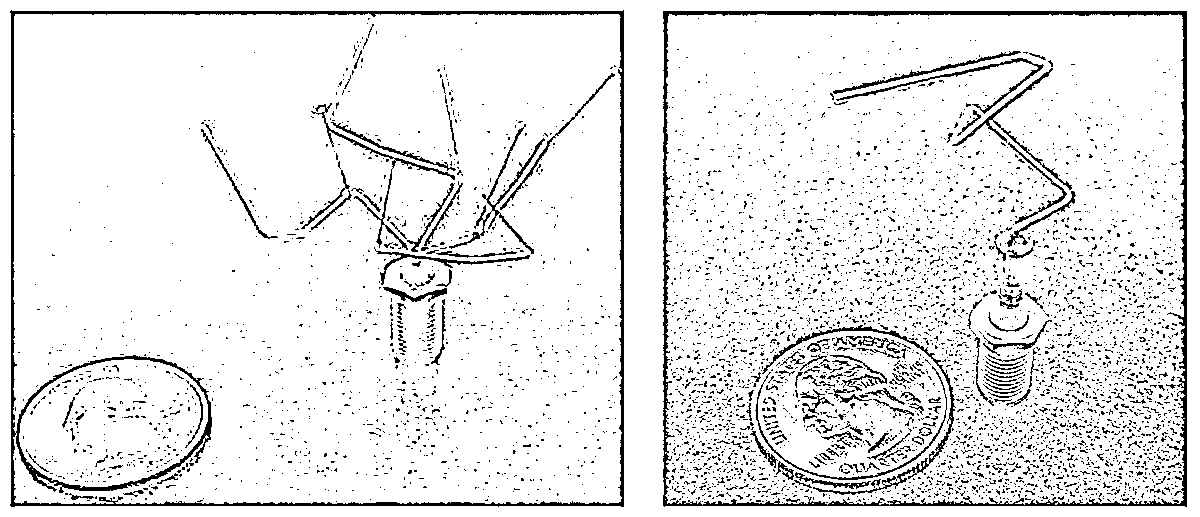
\includegraphics[width=13cm]{GeneticallyGrownAntennas_NASA-web.png} %TODO source 
    \caption{Antennes obtenues par évolution génétique}
\end{figure}

\vspace{-1cm}

\stardelimiter{}

%\vspace{0.36cm}

\newpage

\datemarge{Le}%FIXME

Ah les mardis, quelle épreuve! 
Encore une fois, impossible de rester concentré sur le cours en informatique, malgré mon intérêt pour le sujet!
C'est ce qui arrive lorsque c'est devenu le jour où l'on mange beaucoup entre amis.
Bon, après tout, ca reste assez agréable d'avori cette pause de deux heures le midi: la sensation typique de ne pas avoir de temps des classes préparatoires s'évanouit dans un bon moment de détente et permet d'assurer une forme correcte tous les jours.
Mais je suis totalement incapable de suivre ce cours de logique sans me laisser distraire!
Je regarde le cours qu'on nous a donné: forme normale conjonctive, lois de De Morgan, table de vérité, évaluation\dots
Mouais, c'est quand même pas très sexy comme sujet de toute façon, et ça n'a pas l'air très dur à travailler.
Pendant que je surligne les passages importants sur le cours livré en diapopsitives imprimées, j'essaye d'imaginer de quelle façon présenter mon projet:
il me faut non seulement des idées pour la rendre vivante, avec des expériences et applications concrêtes et sympatique, mais également que je puisse montrer ma connaissance du sujet.
C'est une dure affaire de timing que de faire tout ça en seulement dix minutes, ou quarantes si je réussis à passer les \majuscule{ENS}.
Eventuellement, je n'ai qu'à présenter les résultats en mentionnant que je l'ai résolu avec un algorithme génétique, et présenter d'autres résultats théoriques sur le problème ou encore la convergence du programme?
Ça me donne l'impression de bidouiller ma présentation pour que ça colle à ce qu'on me demande, ça ne me plaît pas trop.
Ou alors, je mentionne plusieurs fois que j'ai travaillé sur le côté théorique et je profite du temps alloué pour les questions pour développer selon ce qui intéresse le jury?
Mmmh, pari risqué encore une fois.

C'est fou que je n'ai toujours pas la moindre idée de comment présenter ça après tout ce temps, même si j'en ai encore beaucoup.

Hop reprise du cours, je parle encore avec mon co-trinôme.
\begin{dialogue}
    \sentence{Ce sont presque que des choses qu'on fait en sciences de l'ingénieur en terminale}.
    \sentence{Oui, je crois même qu'on fait ça en classe de sup aussi.}
    \sentence{En plus, c'est plutôt intuitif. De Morgan, par exemple, c'est juste une histoire de Français.}
    \sentence{Ah, je la connais par c\oe{}ur moi, c'est tout. Je sais juste que c'est ça.}
\end{dialogue}

Il écrit la formule sur le cours pour me la montrer, je suis assez étonné de sa réponse.
%FIXME 
%TODO : afficher la formule
\begin{dialogue}
    \sentence{Mais tu ne l'interprête pas du tout comme du Français?}
    \sentence{Non? Pourquoi, comment est-ce que tu l'interprêtes toi?}
    \sentence{garde, le membre de gauche, c'est que tu n'as aucun de A ou B, et le membre de droite, que tu n'as ni A, ni B. C'est un peu de la distributivité de la négation si tu l'exprimes en Français.}
    \sentence{Ah\dots Oui\dots C'est assez cool en fait! Et tu as déjà vu les tableaux de Karnaugh?}
    \sentence{Carnot? Pour la thermodynamique?}
    \sentence{Non, non, pas ce Carnot-là. Celui pour simplifier les expressions logique.}
    \sentence{Ça me dit quelque chose, peut-être que j'en ai entendu parler en \majuscule{SI} l'année dernière.}
    \sentence{Regarde. Je te le montre avec quatres variables. Avec plus c'est plus vraiment pratique. Tu fais un tableau à deux entrées. Tu mets tes variables ici et là, tu mets le résultat du calcul ici, et tu fais des paquets avec tous les 1 pour avoir la forme simplifiée.}
    \sentence{Euh\dots oui, mais comment tu remplis ce tableau?}
    \sentence{Il suffit de faire le calcul entre les différentes variables.}%TODO
    \sentence{Mmmh, oui, d'accord, et pour les 1, pourquoi tu ne fais pas des lignes de trois 1 ici, ça fait moins de blocs!}
    \sentence{Il faut que ton rectangle ait des côtés de longueur une puissance de deux pour que ça marche, mais par contre ton tableau est comme une sphere, tu peux faire un carré avec les 4 coins ou le commencer sur un bord et prendre l'autre bord avec.}
    \sentence{Mmmh, d'accord.}
\end{dialogue}

J'espère qu'il ne le saura pas, mais je n'ai pas compris grand chose à son tableau. 
Ça ressemble plus à de l'informagie vaudou qu'à une vraie technique de minimisation pour moi, et il y a beaucoup de contraintes étranges sur la réalisation du tableau.
Néanmoins, je garde cette technique en tête, il faudra que je revienne dessus lorsque j'aurais un peu plus de temps.

\datemarge{Le 26 décembre}


\begin{comment}
%TODO: réécrire cette partie
Aujourd'hui, je ne sais vraiment plus quoi faire pour ce projet, rien ne correspond à ce que je veux.
J'ai fini par penser que je n'arriverai pas à terminer à temps.
Il est temps de prendre des mesures pour améliorer cela.
%TODO expliquer pourquoi
Peut être faire un projet en physique, c'est censé être plus facile? Si seulement je pouvais en comprendre quelque chose!
Ou alors un sujet de mathématiques? 
Il faut seulement que je me débarasse de cette impression de ne rien faire moi-même. 

Je suis encore sur Internet, l'autoplay de youtube a fini par m'amener de vidéos d'algorithmes génétiques appliqués au jeu vidéo, à des vidéos de pendule doubles --- à deux tiges --- asservi par un moteur. 
\end{comment}
%FIXME: date, séparer en deux ou pas ?
Enfin les vacances de Nöel, je ne prendrai pas plus de travail en retard que ce que j'ai déjà. 
En revanche, pas le temps de souffler, j'ai beaucoup à faire, et je veux comme cer à programmer le c\oe{}ur du solveur pour le projet.
Mais je ne m'empêche pas de regarder quelques vidéos intéressantes, surtout que c'est à propos de mon sujet favori.
Je regarde une vidéo de démonstration mélangeant réseaux de neurones et algorithmes génétiques afin d'entrainer deux créatures au comportement simplifié à se battre.
%TODO: image + développer

La vidéo suivante m'interpèle également.
Il s'agit encore du même type de système, mais pour entrainer une créature à sauter le plus loin possible, avec des membres définis par l'utilisateur avant la simulation.
C'est assez incroyable de voir à quel point cela fonctionne bien.
Les créatures ne savent rien de leur environnement, et ne savent pas comment elles fonctionnent au début de la simulation, mais finissent par avoir un comportement «rationnel» de manière naturelle.




\helvetica{[SUITE A FAIRE ET RETRAVAILLER]} % TODO
 
\newpage
\hfill\vspace{-0.5cm}
\datemarge{février}
%Les mardis sont souvent une très grande épreuve à vivre. 
%+nourriture
%+ecoute peu attentive
%+parler avec antonin
%+tableau de karnaugh
%+"premiere introduction à la logique"

%\stardelim{}

%


%TODO: ligne horizontal

}
\end{document}
